% This file provides an example Beamer presentation using the RWTH theme
% showcasing some of the more common options, similar to the Powerpoint version
% 12.11.2014: Revision 1 (Harold Bruintjes, Tim Lange)

% For RWTH, beamer should be loaded with class option t (top)
\documentclass[t]{beamer}

% Use fontspec to get Arial font
% Requires use of XeLaTeX
\usepackage{fontspec}
\setmainfont{Arial}
\setsansfont{Arial}
% Also force Arial for math for a more consistent look
\usepackage{unicode-math}

% German style date formatting (footer)
\usepackage[ddmmyyyy]{datetime}
\renewcommand{\dateseparator}{.}

\usepackage{MnSymbol,wasysym}

% Format the captions used for figures etc.
\usepackage[compatibility=false]{caption}
\captionsetup{singlelinecheck=off,justification=raggedleft,labelformat=empty,labelsep=none}

% PGFPlots is used for drawing some of the charts
\usepackage{pgfplots}
\usepackage{blkarray}
\pgfplotsset{compat=newest}
\input{plot_commands.tex}

\setbeamertemplate{bibliography item}{\insertbiblabel}
% Load the actual RWTH theme. Suggested is to load the full theme,
% as it requires some specific dimensions
\usetheme{rwth}

\begin{document}

	\logo{\includegraphics{logo.png}}

% Setup presentation information
	\title{Syntaktische Mehrdeutigkeiten \\ Erkennung, Vermeidung und Auflösung}
	\date{07.06.2024}
	\author{Lennart Protte}

	\frame{\titlepage}


	\section{Motivation}\label{sec:motivation}
	\begin{frame}
		\begin{columns}[T]
			\column{0.5\textwidth}
			\centering
			\begin{block}{Zielsetzung}
				\vspace{1em}
					Entwicklung von Strategien zur \textbf{Erkennung} und \textbf{Lösung} von Mehrdeutigkeiten
					oder zur \textbf{Vermeidung} ihrer Entstehung.
				\vspace{1em}
			\end{block}
			\column{0.5\textwidth}
			\centering
			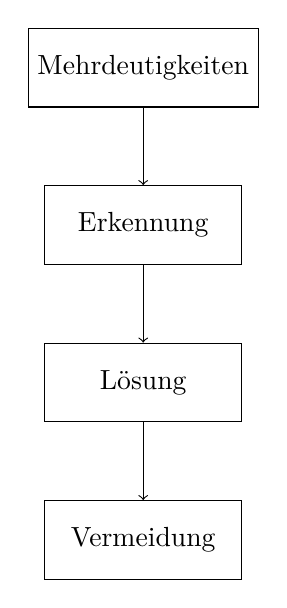
\begin{tikzpicture}[node distance=1.5cm, auto, every node/.style={align=center}]
				% Nodes
				\node (input) [rectangle, draw, text centered, minimum height=1cm, minimum width=2.5cm] {Mehrdeutigkeiten};
				\node (detect) [rectangle, draw, below of=input, text centered, minimum height=1cm, minimum width=2.5cm, yshift=-0.5cm] {Erkennung};
				\node (solve) [rectangle, draw, below of=detect, text centered, minimum height=1cm, minimum width=2.5cm, yshift=-0.5cm] {Lösung};
				\node (avoid) [rectangle, draw, below of=solve, text centered, minimum height=1cm, minimum width=2.5cm, yshift=-0.5cm] {Vermeidung};

				% Arrows
				\draw[->] (input) -- (detect);
				\draw[->] (detect) -- (solve);
				\draw[->] (solve) -- (avoid);
			\end{tikzpicture}

		\end{columns}
	\end{frame}


	\section{Probleme und Herausforderungen}\label{sec:probleme-und-herausforderungen}
	\begin{frame}
		\begin{itemize}
			\item Wann ist ein Syntax Mehrdeutig?
			\item Was ist die Problematik von mehrdeutigen Syntaxen?
			\item Wie können Mehrdeutigkeiten vermieden werden?
			\item Wie können Mehrdeigkeiten erkannt werden?
			\item Wie können Mehrdeutigkeiten aufgelöst werden?
		\end{itemize}
	\end{frame}


	\section{Theoretische Ergebnisse und algorithmische Lösungen}\label{sec:theoretische-ergebnisse-und-algorithmische-losungen}
	\begin{frame}
		\begin{itemize}
			\item Chomsky-NormalForm
			\item Algorithmen zur Erkennung von Mehrdeutigkeiten
			\item Lösungsstrategien: Vorrangsregeln, Assoziativität, Grammatik-Korrektur
		\end{itemize}
		\begin{center}
			\includegraphics[width=\textwidth]{./img}\cite{springer2013}
		\end{center}
	\end{frame}


	\section{Praktische Ansätze}\label{sec:praktische-ansatze}
	\begin{frame}
		\begin{itemize}
			\item Beispiele aus der Praxis: Bekannte Compiler und Programmiersprachen
			\item Fallstudien: Anwendung der Techniken in realen Projekten , (LALR(1), LL(1) Parser)
		\end{itemize}
	\end{frame}


	\section{Ausblick}\label{sec:ausblick-und-zukunftige-projekte}
	\begin{frame}
		\begin{itemize}
			\item Maschinelles Lernen zur Erkennung von Mehrdeutigkeiten
			\item Natürliche Sprache => Komplexe MEhrdeutige Grammatiken
		\end{itemize}
	\end{frame}


	\section{Quellen}\label{sec:quellen}
	\begin{frame}[allowframebreaks]
		\bibliographystyle{apalike}
		\bibliography{refs}
	\end{frame}

\end{document}